\pagechapter{Methodology}
\subsection{Design}
\subsubsection{A guided research journey}
A user selects an asset or hypothetical portfolio and chooses how far ahead to examine risk. EventLens presents relevant events, compares market probabilities with experimental wallet-informed estimates, and lets users inspect wallet activity before exploring scenarios. An AI assistant explains the evidence, and saved reports preserve the analysis.

For example, a user researching SPY over five trading days could inspect an upcoming rate decision, identify which tracked wallets are increasing YES or NO exposure, and compare the resulting risk scenarios. An incompatible announcement horizon or unsupported asset-response estimate will be explained before withholding the affected calculation.

\begin{table}[H]
\smalltable
\caption{Core interface features and the decisions they support.}
\begin{tabularx}{\linewidth}{@{}L{32mm}Y Y@{}}
\toprule\tablehead
\textbf{Screen or feature} & \textbf{What the user sees} & \textbf{What the user can do} \\
\midrule
Overview and watchlist & Supported assets, upcoming eligible events, source freshness and coverage. & Select holdings, choose a horizon and open an event. \\
Event detail & Question, outcome rules, announcement time, market probability and experimental estimate. & Compare estimates and inspect uncertainty and trading activity. \\
Smart-wallet tracker & Tracked addresses, prior event history, YES/NO exposure, recent activity and evidence quality. & Follow wallets, inspect their records and compare their contribution to an event signal. \\
Scenario studio & Gains and losses for each outcome, loss thresholds and average losses in the worst scenarios. & Change a stress assumption or compare paper allocations. \\
Research assistant & An explanation tied to the selected event, portfolio, horizon and evidence. & Ask follow-up questions and open the supporting sources. \\
Saved research & Analysis date, inputs, model and scenario versions, source links and limitations. & Revisit a frozen run and export a readable report with a machine-readable result. \\
\bottomrule
\end{tabularx}
\end{table}

\subsubsection{Smart-wallet tracking and evidence inspection}
Users can browse wallets in covered events, filter by history and activity, and follow public addresses in a research watchlist without connecting a wallet. Profiles show earlier resolved-event decisions, entry prices, subsequent price movements, reconstructed positions and an activity timeline. A provisional ``smart'' label denotes historically informative behaviour, supported by a dated score, sample size and coverage assessment.

Within an event, users can compare YES/NO holdings, agreement and whether a few addresses dominate activity. Contributions to the experimental estimate link to sources and blockchain transactions, distinguishing sampled verification from unchecked records. Personal watchlists do not change model-selection rules.

Results show their horizon, as-of time and missing evidence, separating observations from estimates and assumptions. Users can request explanations and save analyses. Insufficient wallet history leaves the adjustment unavailable while retaining supported market information.

\clearpage
\subsubsection{Concept screens}
Figures~\ref{fig:overview-ui} and~\ref{fig:scenario-ui} illustrate the intended layout. They are conceptual interface images. Values are illustrative and do not represent research results.
\begin{figure}[H]
\centering
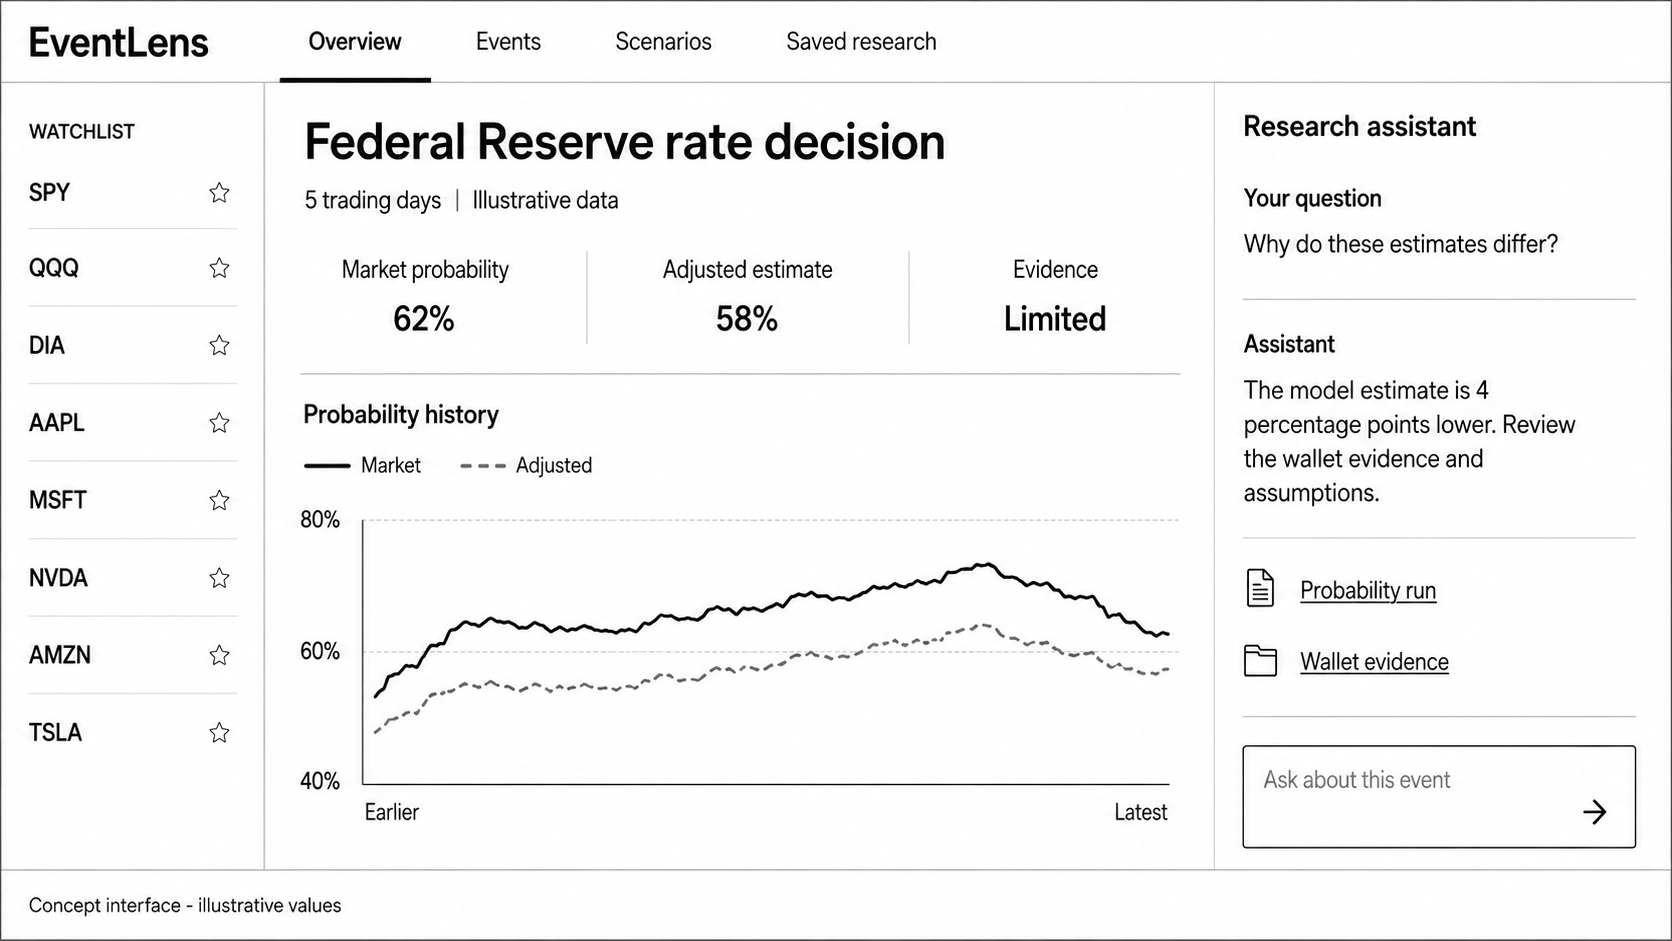
\includegraphics[width=\linewidth]{figures/overview-ui.png}
\caption{Overview concept: a watchlist, event probability comparison and contextual research assistant. All displayed values are illustrative.}
\label{fig:overview-ui}
\end{figure}
\begin{figure}[H]
\centering
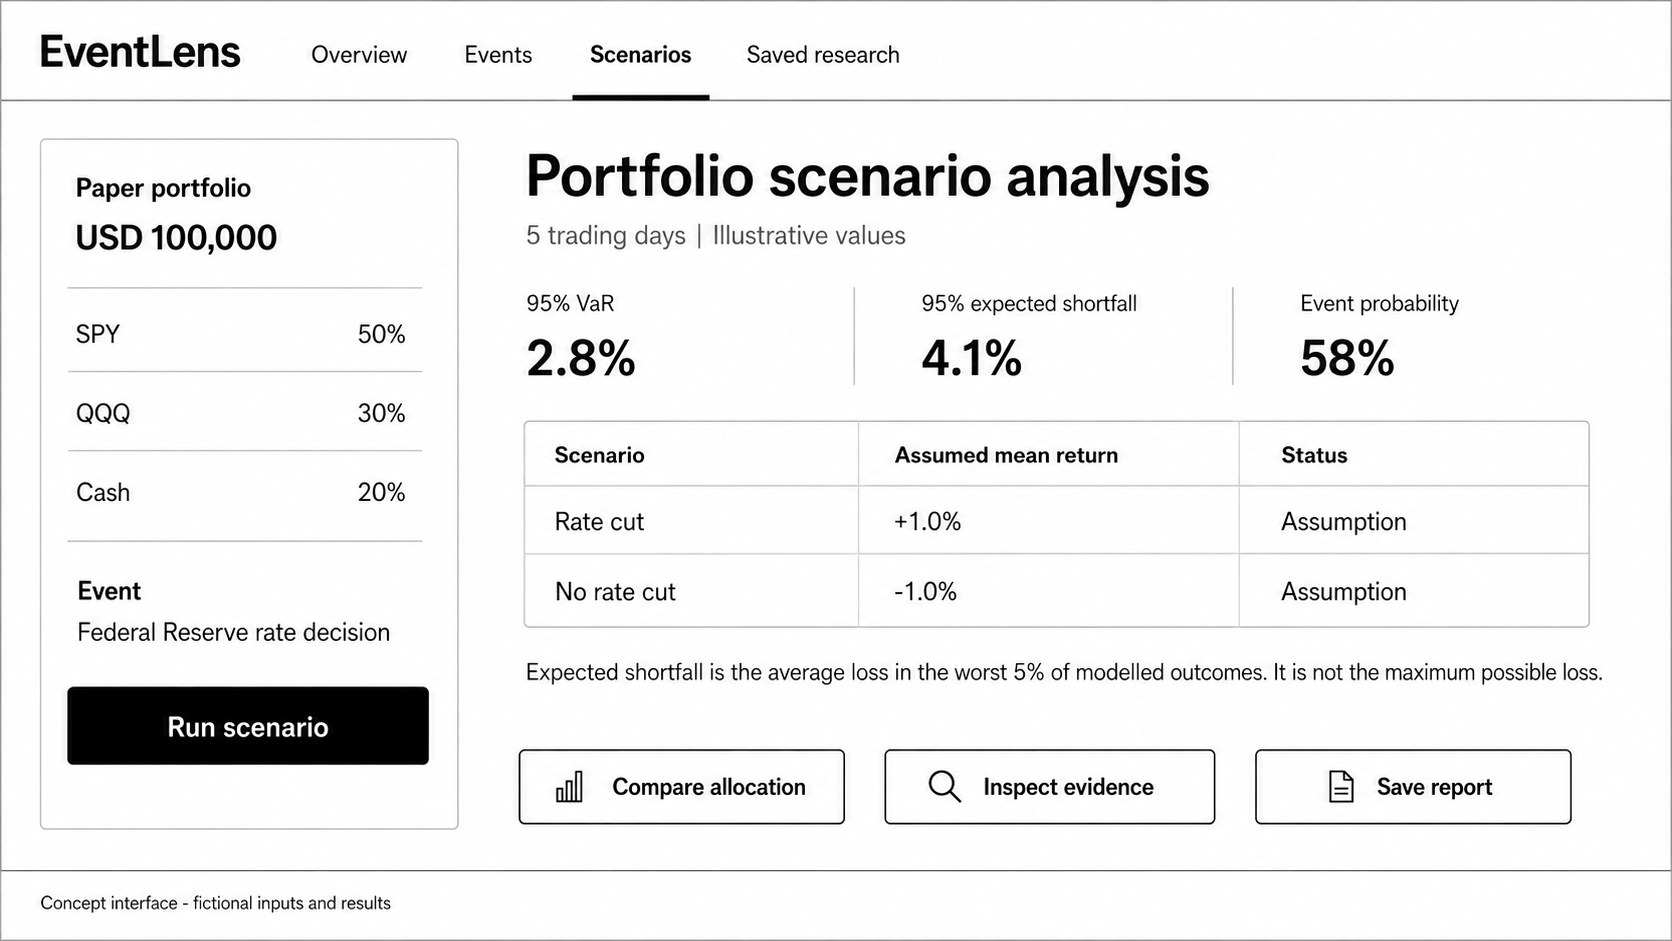
\includegraphics[width=\linewidth]{figures/scenario-ui.png}
\caption{Scenario concept: portfolio inputs, clearly labelled model outputs and visible assumptions. The user compares paper scenarios without placing orders.}
\label{fig:scenario-ui}
\end{figure}
